\documentclass{article}

\usepackage{pgf}
\usepackage{tikz}
\usetikzlibrary{arrows,automata}

\usepackage{lmodern}
\usepackage{amssymb,amsmath}
\usepackage{ifxetex,ifluatex}
\usepackage{multirow}
\usepackage{float}
\usepackage{fixltx2e} % provides \textsubscript
\ifnum 0\ifxetex 1\fi\ifluatex 1\fi=0 % if pdftex
  \usepackage[T1]{fontenc}
  \usepackage[utf8]{inputenc}
\else % if luatex or xelatex
  \ifxetex
    \usepackage{mathspec}
  \else
    \usepackage{fontspec}
  \fi
  \defaultfontfeatures{Ligatures=TeX,Scale=MatchLowercase}
\fi
% use upquote if available, for straight quotes in verbatim environments
\IfFileExists{upquote.sty}{\usepackage{upquote}}{}
% use microtype if available
\IfFileExists{microtype.sty}{%
\usepackage{microtype}
\UseMicrotypeSet[protrusion]{basicmath} % disable protrusion for tt fonts
}{}
\usepackage{hyperref}
\hypersetup{unicode=true,
            pdfborder={0 0 0},
            breaklinks=true}
\urlstyle{same}  % don't use monospace font for urls
\usepackage{color}
\usepackage{fancyvrb}
\newcommand{\VerbBar}{|}
\newcommand{\VERB}{\Verb[commandchars=\\\{\}]}
\DefineVerbatimEnvironment{Highlighting}{Verbatim}{commandchars=\\\{\}}
% Add ',fontsize=\small' for more characters per line
\usepackage{framed}
\definecolor{shadecolor}{RGB}{248,248,248}
\newenvironment{Shaded}{\begin{snugshade}}{\end{snugshade}}
\newcommand{\AlertTok}[1]{\textcolor[rgb]{0.94,0.16,0.16}{#1}}
\newcommand{\AnnotationTok}[1]{\textcolor[rgb]{0.56,0.35,0.01}{\textbf{\textit{#1}}}}
\newcommand{\AttributeTok}[1]{\textcolor[rgb]{0.77,0.63,0.00}{#1}}
\newcommand{\BaseNTok}[1]{\textcolor[rgb]{0.00,0.00,0.81}{#1}}
\newcommand{\BuiltInTok}[1]{#1}
\newcommand{\CharTok}[1]{\textcolor[rgb]{0.31,0.60,0.02}{#1}}
\newcommand{\CommentTok}[1]{\textcolor[rgb]{0.56,0.35,0.01}{\textit{#1}}}
\newcommand{\CommentVarTok}[1]{\textcolor[rgb]{0.56,0.35,0.01}{\textbf{\textit{#1}}}}
\newcommand{\ConstantTok}[1]{\textcolor[rgb]{0.00,0.00,0.00}{#1}}
\newcommand{\ControlFlowTok}[1]{\textcolor[rgb]{0.13,0.29,0.53}{\textbf{#1}}}
\newcommand{\DataTypeTok}[1]{\textcolor[rgb]{0.13,0.29,0.53}{#1}}
\newcommand{\DecValTok}[1]{\textcolor[rgb]{0.00,0.00,0.81}{#1}}
\newcommand{\DocumentationTok}[1]{\textcolor[rgb]{0.56,0.35,0.01}{\textbf{\textit{#1}}}}
\newcommand{\ErrorTok}[1]{\textcolor[rgb]{0.64,0.00,0.00}{\textbf{#1}}}
\newcommand{\ExtensionTok}[1]{#1}
\newcommand{\FloatTok}[1]{\textcolor[rgb]{0.00,0.00,0.81}{#1}}
\newcommand{\FunctionTok}[1]{\textcolor[rgb]{0.00,0.00,0.00}{#1}}
\newcommand{\ImportTok}[1]{#1}
\newcommand{\InformationTok}[1]{\textcolor[rgb]{0.56,0.35,0.01}{\textbf{\textit{#1}}}}
\newcommand{\KeywordTok}[1]{\textcolor[rgb]{0.13,0.29,0.53}{\textbf{#1}}}
\newcommand{\NormalTok}[1]{#1}
\newcommand{\OperatorTok}[1]{\textcolor[rgb]{0.81,0.36,0.00}{\textbf{#1}}}
\newcommand{\OtherTok}[1]{\textcolor[rgb]{0.56,0.35,0.01}{#1}}
\newcommand{\PreprocessorTok}[1]{\textcolor[rgb]{0.56,0.35,0.01}{\textit{#1}}}
\newcommand{\RegionMarkerTok}[1]{#1}
\newcommand{\SpecialCharTok}[1]{\textcolor[rgb]{0.00,0.00,0.00}{#1}}
\newcommand{\SpecialStringTok}[1]{\textcolor[rgb]{0.31,0.60,0.02}{#1}}
\newcommand{\StringTok}[1]{\textcolor[rgb]{0.31,0.60,0.02}{#1}}
\newcommand{\VariableTok}[1]{\textcolor[rgb]{0.00,0.00,0.00}{#1}}
\newcommand{\VerbatimStringTok}[1]{\textcolor[rgb]{0.31,0.60,0.02}{#1}}
\newcommand{\WarningTok}[1]{\textcolor[rgb]{0.56,0.35,0.01}{\textbf{\textit{#1}}}}
\usepackage{graphicx,grffile}
\usepackage{amsmath}

%parte de jhans

%fin de parte de jhans


\title{Predicción de la intensidad de precipitaciones usando el modelo de las cadenas de Markov en la región Áncash}
\author{Juan Andrés Vargas Castillo\\Roosevelt Jhans Ubaldo Chavez}

\begin{document}
\maketitle

\tableofcontents
\newpage

\section{Introducción}

Los autómatas son un modelo computacional muy importante para poder representar distintas distribuciones de un determinado conjunto de símbolos. Un autómata probabilístico es un tipo de autómata en el que se puede observar cual es la probabilidad de que un estado llegue a cualquiera de los otros estados. Estos autómatas están relacionados a las cadenas de Márkov, que se basan en los estados pasados por los que ya paso un sistema para poder predecir a que estado se llegará en el futuro.

A través de las propiedades de las cadenas de Márkov se buscará predecir la intensidad de las futuras precipataciones en la región de Áncash en  el futuro, para esto se usarán las definiciones de autómatas probabilísticos y cadenas de Márkov, así como también los datos meteorológicos previos de la región.

\section{Definición del problema}

Las precipitaciones en las zonas altoandinas de nuestro país son de suma importancia para la siembra y/o cosecha de productos. Una siembra antes de tiempo, podría ocasionar que la planta muera por falta de agua, o en un mayor gasto en riego por parte del agricultor. Del mismo modo, cosechar fuera de tiempo podría ocasionar que se pierda por completo el cultivo, ya que se encuentra en etapa de maduración y ya no requiere agua, de hacerlo podría podrirse la raíz y por ende el fruto. Esto último puede tener un mayor impacto en el cultivo y en la vida del agricultor si se dan las inundaciones a causa de las intensas lluvias.
\\\\
En el presente año, según la Cámara de Comercio de Moquegua, más de 800 héctareas de cultivos fueron perdidas a causa del desborde del río Moquegua ocasionado por las intensas precipitaciones de los últimos meses. Casos similares a este se han venido reportando en los ultimos años en las regiones como Piura, San Martín, Ucayali y Áncash. Es por dicho motivo, que modelar las precipitaciones resultan de suma importancia para la agricultura en nuestro país, así como en acciones para mitigar su impacto.

\section{Marco Teórico}

\subsection{Autómata probabilístico}

\subsubsection{Autómata Finito}
Se define como autómata finito a un modelo computacional, tiene como finalidad reconocer si una entrada o lenguaje pertenece a un conjunto de lenguajes regulares o no. Un autómata también puede ser representado como una 5 - tupla, formada por el conjunto de estados $Q$ a los que puede llegar la entrada, el alfabeto $\Sigma$ con los símbolos que podemos usar para crear nuestros lenguajes, el estado inicial $q_0$ por donde debe empezar el recorrido nuestro lenguaje, la función de transición $\delta$ que nos indica el estado al que llegará un lenguaje al recibir un nuevo símbolo, por último el conjunto de estados finales $F$ que indica si el lenguaje es aceptado o no.

\subsubsection{Autómatas Finitos Deterministas y no Deterministas}

Se tienen dos tipos de autómatas finitos, deterministas y no deterministas. En el primer caso, cuando un símbolo pasa por la función de transición, sólo puede llegar a un estado o a ninguno. Por otro lado, en los no deterministas la función de transición puede retornar más de un estado.

\subsubsection{Definición de un Autómata probabilístico}

Este tipo de autómata se trata de una generalización de un autómata finito no determinista. A diferencia del mencionado, la función de transición no sólo retorna el conjunto de estados a los que se llega con un símbolo, sino que devuelve la propabilidad de llegar a cualquier estado en el autómata. 

\subsection{Cadenas de Márkov}

Las cadenas de Márkov o Sistemas de Márkov son un tipo de autómata probabilístico, en este se busca predecir un posible estado futuro de un sistema. Dicha probabilidad se basa en la historia previa del sistema, esta se encuentra resumida en el estado actual en el que se encuentra. Las cadenas de Márkov tienen diversas aplicaciones en la metereología, modelos epidemiológicos, problemas con simulaciones, genética y más. 

\subsubsection{Probabilidad de Transición}

Se define como probabilidad de transición $P_{ij}$ a la probabilidad que hay de pasar desde un estado $i$ a un estado $j$. El conjunto total de las probabilidades de transición se pueden representar en una matriz de transición.\\
La siguiente matriz representa un Sistema de Márkov con $n$ estados. \\
$$
\begin{bmatrix}
    P_{11}       & P_{12} & P_{13} & \dots & P_{1n} \\
    P_{21}       & P_{22} & P_{23} & \dots & P_{2n} \\
    \hdotsfor{5} \\
    P_{n1}       & P_{n2} & P_{n3} & \dots & P_{nn}
\end{bmatrix}
$$

Cada fila $i$ representa un vector con las probabilidades tal que estamos en el estado $i$, por lo tanto todas las probabilidades de una fila deben sumar 1.

\subsubsection{Vector de Distribución}

Vector con entradas para cada probabilidad de cada estado en un determinado tiempo o número de pasos. La suma de los valores en el vector debe ser igual a 1.\\
El siguiente vector representa una distribución inicial con $n$ estados.

$$
\pi(0) = 
\begin{bmatrix}
    X_{1} & X_{2} & X_{3} & \dots & X_{n}
\end{bmatrix}
$$

Para hallar el siguiente vector de distribución $\pi(1)$ se debe multiplicar el vector de distribución inicial por la matriz de transición.

$$
\pi(1) = \pi(0) * P
$$

$$
\pi(1) = 
\begin{bmatrix}
    X_{1} & X_{2} & X_{3} & \dots & X_{n}
\end{bmatrix}
*
\begin{bmatrix}
    P_{11}       & P_{12} & P_{13} & \dots & P_{1n} \\
    P_{21}       & P_{22} & P_{23} & \dots & P_{2n} \\
    \hdotsfor{5} \\
    P_{n1}       & P_{n2} & P_{n3} & \dots & P_{nn}
\end{bmatrix}
$$

Para hallar $\pi(2)$ debemos multiplicar el vector anterior y multiplicarlo por la matriz de transición.

$$
\pi(2) = \pi(1) * P => \pi(2) = \pi(0) * P^2
$$

Por lo tanto si queremos hallar el vector de distribución $\pi(n)$ después de $n$ pasos.

$$
\pi(n) = \pi(0) * P^n
$$

\subsubsection{Comportamiento a Largo Plazo}
Si para un vector de distribución se cumple que $\pi(n)=\pi(n)*P$ significa que llegamos a vector de estado de equilibrio o vector estabilizado. Por otro lado, una matriz de equilibrio o matriz estabilizada es una matriz donde se cumple $P = P*P$ donde además cada fila es igual a las demás.\\
Para hallar un vector de distribución a largo plazo, vamos potenciando nuestra matriz de transición hasta llegar a una potencia que representa una matriz estabilizada. \\

Ejemplo:\\

Si tenemos la siguiente matriz de transición: 

$$
P = 
\begin{bmatrix}
    0.2       & 0.8 & 0 \\
    0.4       & 0 & 0.6 \\
    0.5       & 0.5 & 0 
\end{bmatrix}
$$

Al calcular $P^{256}$ llegaremos a la matriz de transición estabilizada:

$$
P = 
\begin{bmatrix}
    35/99       & 40/99 & 24/99 \\
    35/99       & 40/99 & 24/99 \\
    35/99       & 40/99 & 24/99 
\end{bmatrix}
$$

\subsection{Ejemplo del Clima}

Dado un pueblo donde el clima puede cambiar de un día para otro: 

\begin{itemize}
    \item El clima sólo puede ser o húmedo o seco.
    \item Si el día actual es seco, la probabilidad de que mañana sea seco es de 80\%.
    \item Si el día actual es húmedo, la probabilidad de que mañana sea seco es de 60\%.
\end{itemize}
$$X = EstadoDelClima.$$
$$
X = 
\begin{Bmatrix}
    0 & seco \\
    1 & húmedo
\end{Bmatrix}
$$

\begin{enumerate}
\item{Matriz de transicción}

\begin{table}[htbp]
\begin{center}
\begin{tabular}{|l|l|l}
\hline
\hline
\multicolumn{1}{|c|}{\multirow{2}{*}{\textbf{Estado Actual X}}} & \multicolumn{2}{c|}{\textbf{Estado Siguiente X}} \\ \cline{2-3} 
\multicolumn{1}{|c|}{}                      & 0                     & 1                     \\ \hline
0                                           & $P_{00}=0.8$          & $P_{01}=0.2$          \\ \hline
1                                           & $P_{10}=0.6$          & $P_{11}=0.4$          \\ \hline

\end{tabular}
\caption{Matriz de transición}
\label{tabla:mtransicion}
\end{center}
\end{table}

\item{Diagrama de transición}\\
\begin{center}
\begin{tikzpicture}[->,>=stealth',shorten >=1pt,auto,node distance=2.8cm,
                    semithick]
  \tikzstyle{every state}=[fill=white,draw=black,text=black]

    \node[state] (B)  {$0$};
    \node[state] (C) [right of=B] {$1$};
    
    \path[->] (B)         edge [loop above] node {$0.8$} ()
           (B)         edge [bend left]  node {$0.2$} (C)
           (C)         edge [bend left]  node {$0.6$} (B)
           (C)         edge [loop below] node {$0.4$} ()
\end{tikzpicture}
\end{center}
\end{enumerate}




\section{Estado del Arte}

\subsection{Forecasting of meteorological drought using Hidden Markov Model}

En este estudio, a través de un modelo homogéneo de Markov oculto, se busca pronosticar sequías en base a al índice de precipitación estandarizado, a corto y mediano plazo. Para medir el rendimiento de este modelo  se usaron varios criterios de pronóstico. Los resultados parecen validar la fiabilidad del modelo usado para pronosticar posibles eventos con las sequías.

\subsection{Markov chain analysis of the rainfall patterns of five geographical locations in the south eastern coast of Ghana}

Este estudio realiza un análisis de Márkov usando datos de lluvias registradas por día entre los años 1980 y 2010 en las siguientes ciudades pertenecientes a la costa sudeste de Ghana; Costa del Cabo, Accra, Akuse, Akatsi y Keta. Se calculan las matrices de transición para cada ciudad y mes usando la probabilidad condicional de si en un día hubo o no lluvia. De los resultados se concluyó que para Accra, la temporada de lluvias era en los meses de mayo a junio y de septiembre a octubre. También determinamos que la probabilidad de lluvia generalmente tiende a aumentar de este a oeste a lo largo de la costa sureste de Ghana.

\subsection{Markov Chain Model and Its Application to Annual Rainfall Distribution for Crop Production}

Este estudio trabaja con distintos estados y tiempos a través del uso de cádenas de Márkov. A través de este principio se plantea un modelo de cuatro estados para la distribución anual de lluvias en Minna con respecto a la producción de cultivos. Con este modelo, podemos recibir el estado de un determinado año y en base a este poder determinar la probabilidad de hacer una transición a cualquiera de los otros estados. El modelo provee información sobre las lluvias en relación a los cultivos que puede ser usada tanto por campesinos como por el gobierno. 

\section{Propuesta}

En el presente artículo se van a analizar las presencia de precipitaciones en la región de Áncash mediante el uso de las cadenas de Markov. La data a usar en este estudio será recopilada de 3 estaciones metereologícas del SENAHMI dispersas a lo largo de la región (Milpo, Recuay y Pira). Los meses considerados para el estudio corresponden al periodo de siembra del maíz entre los meses de marzo-abril y su respectiva cosecha entre julio-agosto del 2018. Se uso el maíz como referencia, ya que es uno de los productos con mayor volumén de producción en la región. 
\\\\
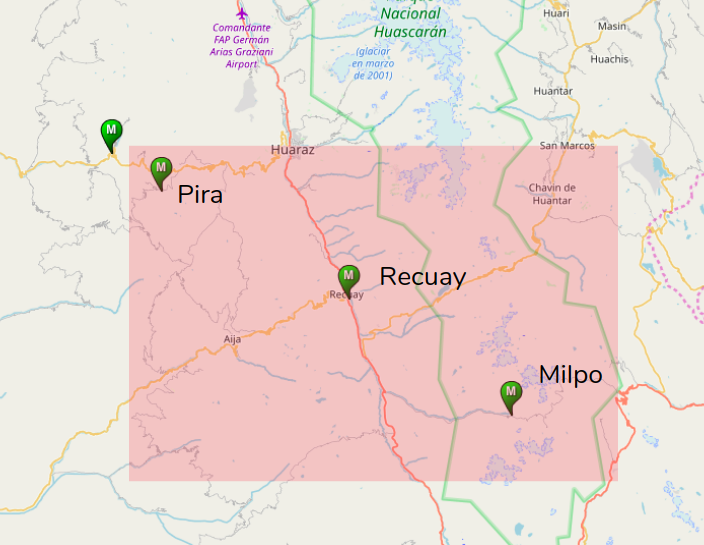
\includegraphics[width=\textwidth]{mapa.png}\\\\

Se modelará la cadena de Markov mediante una autómata probabilística de tres estados seco, húmedo y lluvioso.



\section{Cálculo de las matrices de transición}
%jhans

Se realizaron los cálculos de la matriz de transición para los puesto
metereológicos de Milpo, Pira y Recuay. Todos ellos dentro del
departamento de Ancash. El proceso se realizó haciendo uso de R y se
detalla a continuación:

Los dataset fueron extraídos de la página web del Senahmi.

\begin{Shaded}
\begin{Highlighting}[]
\CommentTok{#Cargar los datasets}
\NormalTok{milpo<-}\KeywordTok{read.table}\NormalTok{(}\StringTok{"milpo.txt"}\NormalTok{, }\DataTypeTok{header =} \OtherTok{FALSE}\NormalTok{, }\DataTypeTok{sep =} \StringTok{" "}\NormalTok{, }\DataTypeTok{dec =}\StringTok{"."}\NormalTok{)}
\NormalTok{pira<-}\KeywordTok{read.table}\NormalTok{(}\StringTok{"pira.txt"}\NormalTok{, }\DataTypeTok{header =} \OtherTok{FALSE}\NormalTok{, }\DataTypeTok{sep =} \StringTok{" "}\NormalTok{, }\DataTypeTok{dec =}\StringTok{"."}\NormalTok{)}
\NormalTok{recuay<-}\KeywordTok{read.table}\NormalTok{(}\StringTok{"recuay.txt"}\NormalTok{, }\DataTypeTok{header =} \OtherTok{FALSE}\NormalTok{, }\DataTypeTok{sep =} \StringTok{" "}\NormalTok{, }\DataTypeTok{dec =} \StringTok{"."}\NormalTok{)}
\end{Highlighting}
\end{Shaded}

\begin{Shaded}
\begin{Highlighting}[]
\CommentTok{#Cambiar los datos faltantes por NA}
\NormalTok{milpo[milpo}\OperatorTok{==-}\FloatTok{99.9}\NormalTok{]<-}\OtherTok{NA}
\NormalTok{pira[pira}\OperatorTok{==-}\FloatTok{99.9}\NormalTok{]<-}\OtherTok{NA}
\NormalTok{recuay[recuay}\OperatorTok{==-}\FloatTok{99.9}\NormalTok{]<-}\OtherTok{NA}
\end{Highlighting}
\end{Shaded}

A continuación se muestran gráficos que resumen la data que se está
utilizando:\\\\

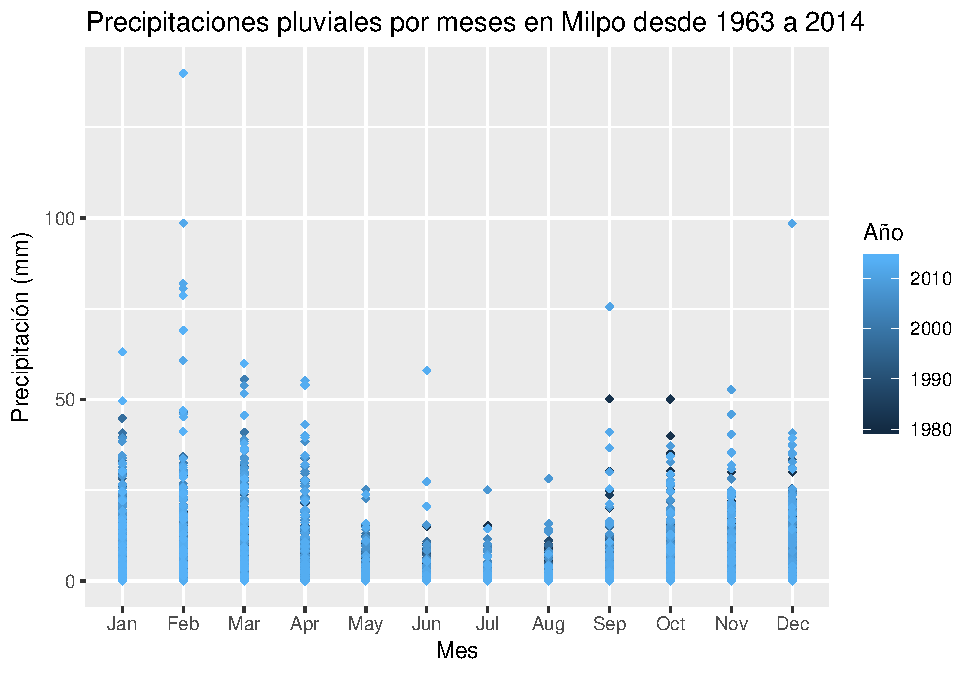
\includegraphics[width=\textwidth]{proyecto_files/unnamed-chunk-5-1.pdf}\\\\
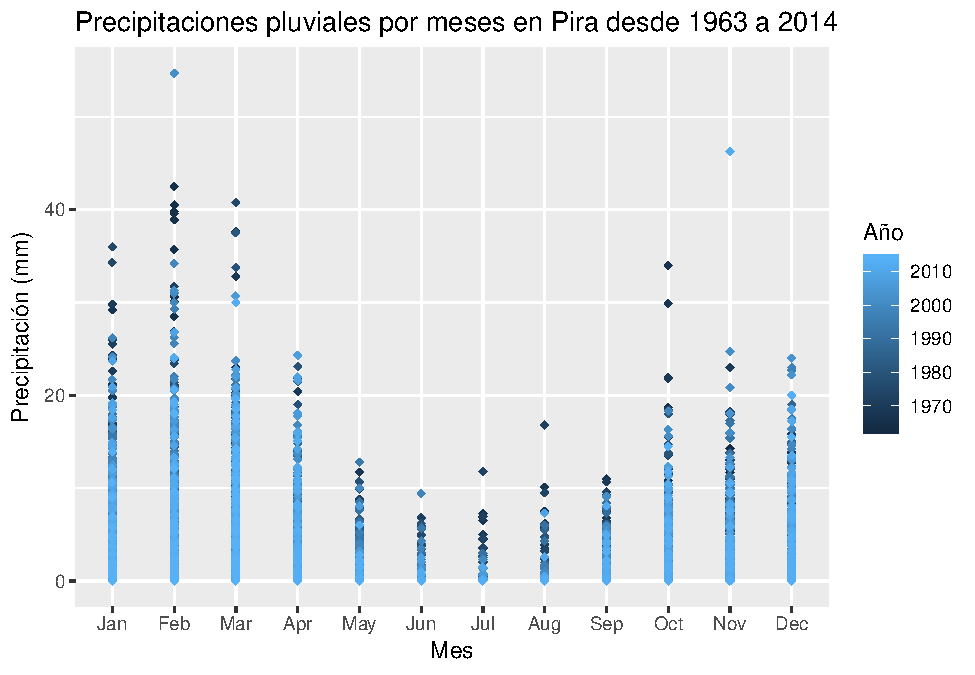
\includegraphics[width=\textwidth]{proyecto_files/unnamed-chunk-5-2.pdf}\\\\
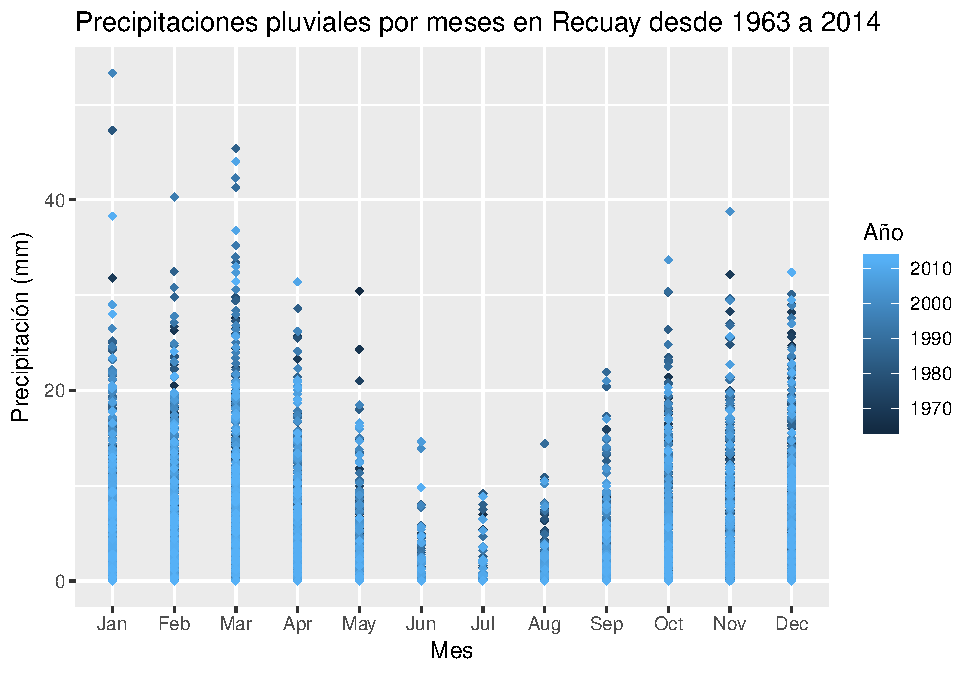
\includegraphics[width=\textwidth]{proyecto_files/unnamed-chunk-5-3.pdf}\\\\
También se genera un gráfico de un año promedio para cada una de las
estaciones metereológicas consideradas en el estudio:\\\\
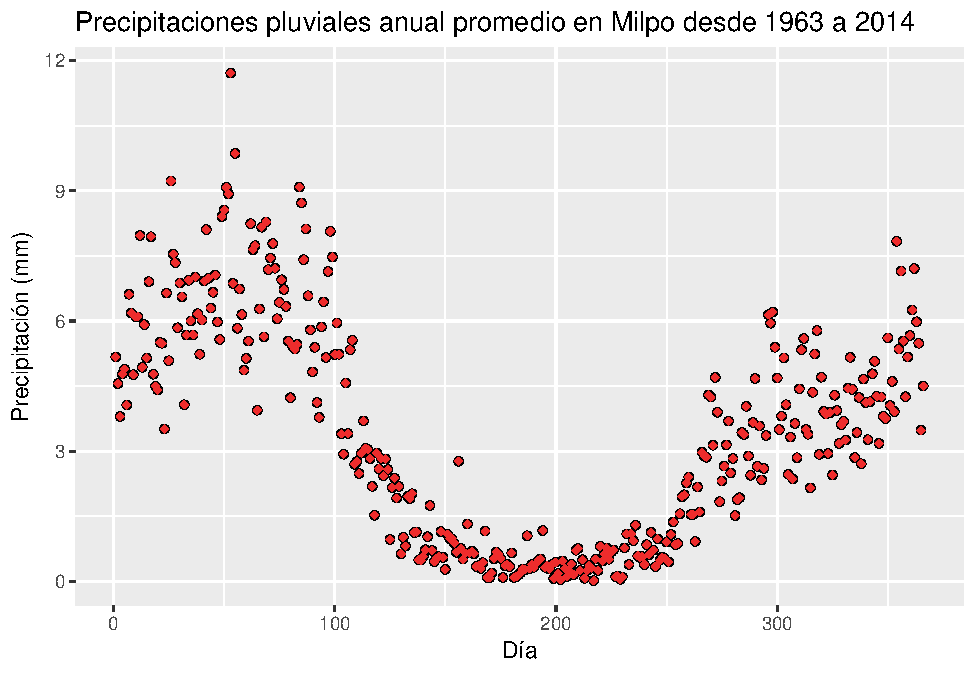
\includegraphics[width=\textwidth]{proyecto_files/unnamed-chunk-6-1.pdf}\\\\
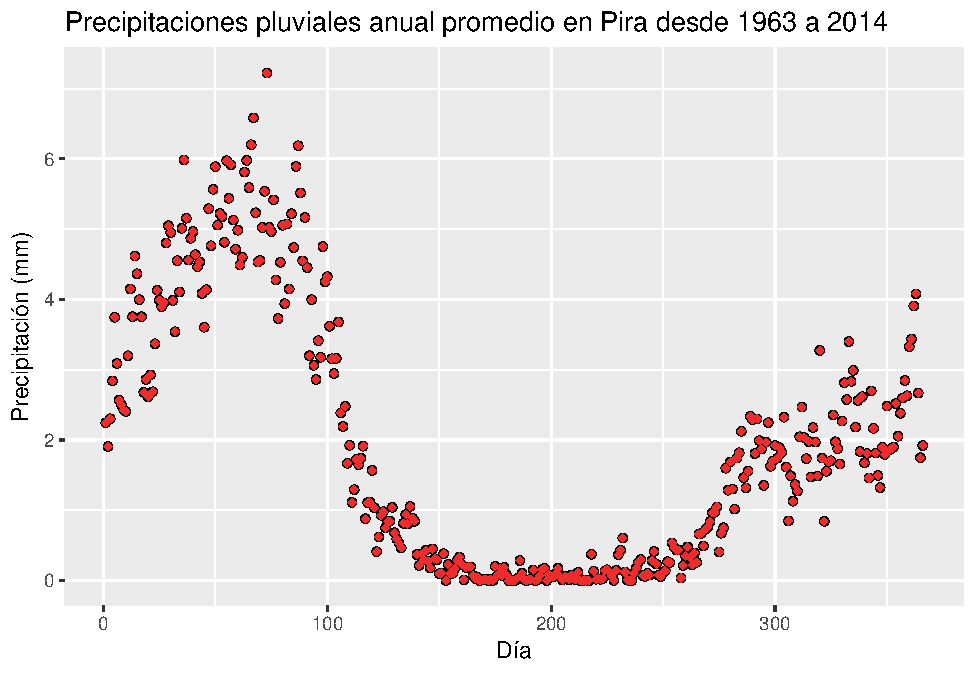
\includegraphics[width=\textwidth]{proyecto_files/unnamed-chunk-6-2.pdf}\\\\
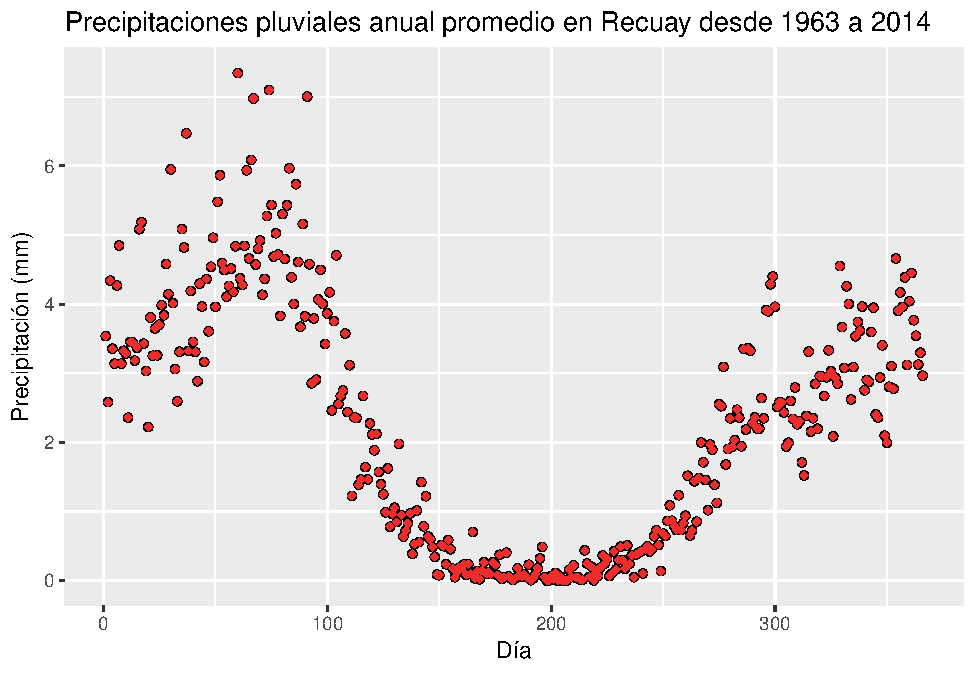
\includegraphics[width=\textwidth]{proyecto_files/unnamed-chunk-6-3.pdf}\\\\

\hypertarget{matrices-de-transicion}{%
\subsection{Matrices de transición}\label{matrices-de-transicion}}
Para realizar la matriz transición se consideraron tres estados: seco, húmedo y
lluvioso. El criterio para clasificar un día dentro de estos estados se base en la clasificación de las lluvias según su intensidad.

\begin{table}[H]
\caption{Clasificación de las precipitaciones según su intensidad}
\begin{center}
\begin{tabular}{|c|c|}
\hline
\textbf{Intensidad} & \textbf{mm/h} \\ \hline
Ligera & $<2.5$  \\ \hline
Moderada & $2.5$ - $7.5$  \\ \hline
Fuerte & $>7.5$ \\ \hline
\multicolumn{2}{l}{$^{\mathrm{Fuente:García, J. (2004)}}$}
\end{tabular}
\label{tab1}
\end{center}
\end{table}



\begin{table}[H]
\caption{Criterio de clasificación de los estados}
\begin{center}
\begin{tabular}{|c|c|c|}
\hline
\textbf{Intensidad} & \textbf{Estado} & \textbf{Nomenclatura} \\ \hline
Ligera & Seco & \textit{s} \\ \hline
Moderada & Húmedo & \textit{h} \\ \hline
Fuerte & Lluvioso & \textit{l} \\ \hline
\end{tabular}
\label{tab1}
\end{center}
\end{table}

A partir de lo anterior se escogieron los siguientes estados de transición y se les asignó un número distintivo. 

\begin{itemize}
\tightlist
\item
  Ayer fue seco y hoy fue seco \(P_{ss}\): \(1\)
\item
  Ayer fue seco y hoy fue húmedo \(P_{sh}\): \(2\)
\item
  Ayer fue seco y hoy fue lluvioso \(P_{sl}\): \(3\)
\item
  Ayer fue húmedo y hoy fue seco \(P_{hs}\): \(4\)
\item
  Ayer fue húmedo y hoy fue húmedo \(P_{hh}\): \(5\)
\item
  Ayer fue húmedo y hoy fue lluvioso \(P_{hl}\): \(6\)
\item
  Ayer fue lluvioso y hoy fue seco \(P_{ls}\): \(7\)
\item
  Ayer fue lluvioso y hoy fue húmedo \(P_{lh}\): \(8\)
\item
  Ayer fue lluvioso y hoy fue lluvioso \(P_{ll}\): \(9\)
\end{itemize}

\begin{center}
    \begin{tikzpicture}[%
     >=stealth,
     shorten >=1pt,
     node distance=4cm,
     on grid,
     auto,
     state/.append style={minimum size=2em},
     thick
   ]
     \node[state] (A)              {$s$};
     \node[state] (B) [below left of=A] {$h$};
     \node[state] (C) [below right of=A] {$l$};
 
     \path[->] 
               (A)         edge [loop above] node {$P_{ss}$} ()
               (A)         edge   node {$P_{sh}$} (B)
               (A)         edge [bend left]  node {$P_{sl}$} (C)
               (B)         edge [bend left]  node {$P_{hs}$} (A)
               (B)         edge   node {$P_{hl}$} (C)
               (B)         edge [loop below] node {$P_{hh}$} ()
               (C)         edge [bend left]  node {$P_{lh}$} (B)
               (C)         edge   node {$P_{ls}$} (A)
               (C)         edge [loop below] node {$P_{ll}$} ()
   \end{tikzpicture}
\end{center}

Por lo tanto, la \textbf{matriz de transición:} será una matriz de $3 \times 3$ como se muestra a continuación: 


\[M=\left( \begin{array}{cccc}
 P_{ss} & P_{sh} & P_{sl}\\ 
 P_{hs} & P_{hh} & P_{hl} \\
 P_{ls} & P_{lh} & P_{ll}
\end{array} \right)\]

La siguiente función se hizo para determinar los estados antes
mencionados:

\begin{Shaded}
\begin{Highlighting}[]
\CommentTok{# Determinación de estados}
\NormalTok{conteoCasos<-}\ControlFlowTok{function}\NormalTok{ (data)\{}
\NormalTok{  data}\OperatorTok{$}\NormalTok{V4[data}\OperatorTok{$}\NormalTok{V4}\OperatorTok{<}\FloatTok{2.5}\NormalTok{]<-}\DecValTok{0} 
\NormalTok{  data}\OperatorTok{$}\NormalTok{V4[data}\OperatorTok{$}\NormalTok{V4}\OperatorTok{>=}\FloatTok{2.5} \OperatorTok{&}\StringTok{ }\NormalTok{data}\OperatorTok{$}\NormalTok{V4}\OperatorTok{<}\FloatTok{7.5}\NormalTok{]<-}\DecValTok{1}
\NormalTok{  data}\OperatorTok{$}\NormalTok{V4[data}\OperatorTok{$}\NormalTok{V4}\OperatorTok{>=}\FloatTok{7.5}\NormalTok{]<-}\DecValTok{2}
\NormalTok{  tot<-data }\OperatorTok\StringTok{ }\KeywordTok{select}\NormalTok{(}\OperatorTok{-}\NormalTok{V6) }\OperatorTok\StringTok{ }\KeywordTok{filter}\NormalTok{(V4 }\OperatorTok{==}\StringTok{ }\DecValTok{0} \OperatorTok{|}\StringTok{ }\NormalTok{V4 }\OperatorTok{==}\StringTok{ }\DecValTok{1} \OperatorTok{|}\StringTok{ }\NormalTok{V4 }\OperatorTok{==}\StringTok{ }\DecValTok{2}\NormalTok{) }\CommentTok{##obviamos NAs}
\NormalTok{  tot}\OperatorTok{$}\NormalTok{V5[}\DecValTok{1}\NormalTok{]<-}\DecValTok{0} \CommentTok{#el primer día tiene valor cero}
  \ControlFlowTok{for}\NormalTok{ (i }\ControlFlowTok{in} \DecValTok{2}\OperatorTok{:}\KeywordTok{nrow}\NormalTok{(tot))\{}
    \ControlFlowTok{if}\NormalTok{ (tot}\OperatorTok{$}\NormalTok{V4[i}\DecValTok{-1}\NormalTok{]}\OperatorTok{==}\DecValTok{0} \OperatorTok{&}\StringTok{ }\NormalTok{tot}\OperatorTok{$}\NormalTok{V4[i]}\OperatorTok{==}\DecValTok{0}\NormalTok{)\{ }\CommentTok{#Pss}
\NormalTok{      tot}\OperatorTok{$}\NormalTok{V5[i]<-}\DecValTok{1}
\NormalTok{    \} }\ControlFlowTok{else} \ControlFlowTok{if}\NormalTok{(tot}\OperatorTok{$}\NormalTok{V4[i}\DecValTok{-1}\NormalTok{]}\OperatorTok{==}\DecValTok{0} \OperatorTok{&}\StringTok{ }\NormalTok{tot}\OperatorTok{$}\NormalTok{V4[i]}\OperatorTok{==}\DecValTok{1}\NormalTok{)\{ }\CommentTok{#Psh}
\NormalTok{      tot}\OperatorTok{$}\NormalTok{V5[i]<-}\DecValTok{2}
\NormalTok{    \} }\ControlFlowTok{else} \ControlFlowTok{if}\NormalTok{ (tot}\OperatorTok{$}\NormalTok{V4[i}\DecValTok{-1}\NormalTok{]}\OperatorTok{==}\DecValTok{0} \OperatorTok{&}\StringTok{ }\NormalTok{tot}\OperatorTok{$}\NormalTok{V4[i]}\OperatorTok{==}\DecValTok{2}\NormalTok{)\{ }\CommentTok{#Psl}
\NormalTok{      tot}\OperatorTok{$}\NormalTok{V5[i]<-}\DecValTok{3}
\NormalTok{    \}}\ControlFlowTok{else} \ControlFlowTok{if}\NormalTok{(tot}\OperatorTok{$}\NormalTok{V4[i}\DecValTok{-1}\NormalTok{]}\OperatorTok{==}\DecValTok{1} \OperatorTok{&}\StringTok{ }\NormalTok{tot}\OperatorTok{$}\NormalTok{V4[i]}\OperatorTok{==}\DecValTok{0}\NormalTok{)\{ }\CommentTok{#Phs}
\NormalTok{      tot}\OperatorTok{$}\NormalTok{V5[i]<-}\DecValTok{4}
\NormalTok{    \}}\ControlFlowTok{else} \ControlFlowTok{if}\NormalTok{(tot}\OperatorTok{$}\NormalTok{V4[i}\DecValTok{-1}\NormalTok{]}\OperatorTok{==}\DecValTok{1} \OperatorTok{&}\StringTok{ }\NormalTok{tot}\OperatorTok{$}\NormalTok{V4[i]}\OperatorTok{==}\DecValTok{1}\NormalTok{)\{ }\CommentTok{#Phh}
\NormalTok{      tot}\OperatorTok{$}\NormalTok{V5[i]<-}\DecValTok{5}
\NormalTok{    \}}\ControlFlowTok{else} \ControlFlowTok{if}\NormalTok{(tot}\OperatorTok{$}\NormalTok{V4[i}\DecValTok{-1}\NormalTok{]}\OperatorTok{==}\DecValTok{1} \OperatorTok{&}\StringTok{ }\NormalTok{tot}\OperatorTok{$}\NormalTok{V4[i]}\OperatorTok{==}\DecValTok{2}\NormalTok{)\{ }\CommentTok{#Phl}
\NormalTok{      tot}\OperatorTok{$}\NormalTok{V5[i]<-}\DecValTok{6}
\NormalTok{    \}}\ControlFlowTok{else} \ControlFlowTok{if}\NormalTok{(tot}\OperatorTok{$}\NormalTok{V4[i}\DecValTok{-1}\NormalTok{]}\OperatorTok{==}\DecValTok{2} \OperatorTok{&}\StringTok{ }\NormalTok{tot}\OperatorTok{$}\NormalTok{V4[i]}\OperatorTok{==}\DecValTok{0}\NormalTok{)\{ }\CommentTok{#Pls}
\NormalTok{      tot}\OperatorTok{$}\NormalTok{V5[i]<-}\DecValTok{7}
\NormalTok{    \}}\ControlFlowTok{else} \ControlFlowTok{if}\NormalTok{(tot}\OperatorTok{$}\NormalTok{V4[i}\DecValTok{-1}\NormalTok{]}\OperatorTok{==}\DecValTok{2} \OperatorTok{&}\StringTok{ }\NormalTok{tot}\OperatorTok{$}\NormalTok{V4[i]}\OperatorTok{==}\DecValTok{1}\NormalTok{)\{ }\CommentTok{#Plh}
\NormalTok{      tot}\OperatorTok{$}\NormalTok{V5[i]<-}\DecValTok{8}
\NormalTok{    \}}\ControlFlowTok{else} \ControlFlowTok{if}\NormalTok{(tot}\OperatorTok{$}\NormalTok{V4[i}\DecValTok{-1}\NormalTok{]}\OperatorTok{==}\DecValTok{2} \OperatorTok{&}\StringTok{ }\NormalTok{tot}\OperatorTok{$}\NormalTok{V4[i]}\OperatorTok{==}\DecValTok{2}\NormalTok{)\{ }\CommentTok{#Pll}
\NormalTok{      tot}\OperatorTok{$}\NormalTok{V5[i]<-}\DecValTok{9}
\NormalTok{    \}}
    
\NormalTok{  \}}
  \KeywordTok{return}\NormalTok{ (tot)}
\NormalTok{\}}
\end{Highlighting}
\end{Shaded}

\begin{Shaded}
\begin{Highlighting}[]
\CommentTok{# Función que verifica que existan valores en los meses, si no lo hay los rellena con ceros}
\NormalTok{check <-}\StringTok{ }\ControlFlowTok{function}\NormalTok{ (data)\{}
\NormalTok{  dif <-}\StringTok{ }\KeywordTok{setdiff}\NormalTok{(}\KeywordTok{c}\NormalTok{(}\DecValTok{1}\OperatorTok{:}\DecValTok{12}\NormalTok{),}\KeywordTok{c}\NormalTok{(data}\OperatorTok{$}\NormalTok{V2))}
  \ControlFlowTok{if}\NormalTok{ (}\KeywordTok{length}\NormalTok{(dif)}\OperatorTok{>=}\DecValTok{1}\NormalTok{)\{}
    \ControlFlowTok{for}\NormalTok{(i }\ControlFlowTok{in}\NormalTok{ dif)\{}
\NormalTok{      data <-}\StringTok{ }\KeywordTok{rbind}\NormalTok{(data, }\KeywordTok{c}\NormalTok{(i, }\DecValTok{0}\NormalTok{))}
\NormalTok{    \}}
\NormalTok{  \}}
\NormalTok{  data <-}\StringTok{ }\NormalTok{data[}\KeywordTok{order}\NormalTok{(data}\OperatorTok{$}\NormalTok{V2),]}
  \KeywordTok{return}\NormalTok{(data)}
\NormalTok{\}}
\end{Highlighting}
\end{Shaded}

\begin{Shaded}
\begin{Highlighting}[]
\CommentTok{#Función de conteo y probabilidad de cada estado de la matriz de transición}
\NormalTok{probabilidades<-}\ControlFlowTok{function}\NormalTok{(data)\{}
\NormalTok{  dta <-}\StringTok{ }\KeywordTok{conteoCasos}\NormalTok{(data) }\OperatorTok\StringTok{ }\KeywordTok{filter}\NormalTok{(V5 }\OperatorTok{!=}\DecValTok{0}\NormalTok{) }\CommentTok{#eliminamos primer día}
\NormalTok{    uno <-dta }\OperatorTok\StringTok{ }\KeywordTok{group_by}\NormalTok{(V2) }\OperatorTok\StringTok{ }\KeywordTok{filter}\NormalTok{(V5}\OperatorTok{==}\DecValTok{1}\NormalTok{) }\OperatorTok\StringTok{ }\KeywordTok{summarise}\NormalTok{(}\DataTypeTok{uno=}\KeywordTok{n}\NormalTok{()) }\OperatorTok\StringTok{ }\NormalTok{check}
\NormalTok{    dos <-dta }\OperatorTok\StringTok{ }\KeywordTok{group_by}\NormalTok{(V2) }\OperatorTok\StringTok{ }\KeywordTok{filter}\NormalTok{(V5}\OperatorTok{==}\DecValTok{2}\NormalTok{) }\OperatorTok\StringTok{ }\KeywordTok{summarise}\NormalTok{(}\DataTypeTok{dos=}\KeywordTok{n}\NormalTok{()) }\OperatorTok\StringTok{ }\NormalTok{check}
\NormalTok{    tres <-dta }\OperatorTok\StringTok{ }\KeywordTok{group_by}\NormalTok{(V2) }\OperatorTok\StringTok{ }\KeywordTok{filter}\NormalTok{(V5}\OperatorTok{==}\DecValTok{3}\NormalTok{) }\OperatorTok\StringTok{ }\KeywordTok{summarise}\NormalTok{(}\DataTypeTok{tres=}\KeywordTok{n}\NormalTok{()) }\OperatorTok\StringTok{ }\NormalTok{check}
\NormalTok{    cuatro <-dta }\OperatorTok\StringTok{ }\KeywordTok{group_by}\NormalTok{(V2) }\OperatorTok\StringTok{ }\KeywordTok{filter}\NormalTok{(V5}\OperatorTok{==}\DecValTok{4}\NormalTok{) }\OperatorTok\StringTok{ }\KeywordTok{summarise}\NormalTok{(}\DataTypeTok{cuatro=}\KeywordTok{n}\NormalTok{()) }\OperatorTok\StringTok{ }\NormalTok{check}
\NormalTok{    cinco <-dta }\OperatorTok\StringTok{ }\KeywordTok{group_by}\NormalTok{(V2) }\OperatorTok\StringTok{ }\KeywordTok{filter}\NormalTok{(V5}\OperatorTok{==}\DecValTok{5}\NormalTok{) }\OperatorTok\StringTok{ }\KeywordTok{summarise}\NormalTok{(}\DataTypeTok{cinco=}\KeywordTok{n}\NormalTok{()) }\OperatorTok\StringTok{ }\NormalTok{check}
\NormalTok{    seis <-dta }\OperatorTok\StringTok{ }\KeywordTok{group_by}\NormalTok{(V2) }\OperatorTok\StringTok{ }\KeywordTok{filter}\NormalTok{(V5}\OperatorTok{==}\DecValTok{6}\NormalTok{) }\OperatorTok\StringTok{ }\KeywordTok{summarise}\NormalTok{(}\DataTypeTok{seis=}\KeywordTok{n}\NormalTok{()) }\OperatorTok\StringTok{ }\NormalTok{check}
\NormalTok{    siete <-dta }\OperatorTok\StringTok{ }\KeywordTok{group_by}\NormalTok{(V2) }\OperatorTok\StringTok{ }\KeywordTok{filter}\NormalTok{(V5}\OperatorTok{==}\DecValTok{7}\NormalTok{) }\OperatorTok\StringTok{ }\KeywordTok{summarise}\NormalTok{(}\DataTypeTok{siete=}\KeywordTok{n}\NormalTok{()) }\OperatorTok\StringTok{ }\NormalTok{check}
\NormalTok{    ocho <-dta }\OperatorTok\StringTok{ }\KeywordTok{group_by}\NormalTok{(V2) }\OperatorTok\StringTok{ }\KeywordTok{filter}\NormalTok{(V5}\OperatorTok{==}\DecValTok{8}\NormalTok{) }\OperatorTok\StringTok{ }\KeywordTok{summarise}\NormalTok{(}\DataTypeTok{ocho=}\KeywordTok{n}\NormalTok{()) }\OperatorTok\StringTok{ }\NormalTok{check}
\NormalTok{    nueve <-dta }\OperatorTok\StringTok{ }\KeywordTok{group_by}\NormalTok{(V2) }\OperatorTok\StringTok{ }\KeywordTok{filter}\NormalTok{(V5}\OperatorTok{==}\DecValTok{9}\NormalTok{) }\OperatorTok\StringTok{ }\KeywordTok{summarise}\NormalTok{(}\DataTypeTok{nueve=}\KeywordTok{n}\NormalTok{()) }\OperatorTok\StringTok{ }\NormalTok{check}
    
\NormalTok{    a<-dta }\OperatorTok\StringTok{ }\KeywordTok{group_by}\NormalTok{(V2) }\OperatorTok\StringTok{ }\KeywordTok{filter}\NormalTok{(V5}\OperatorTok{==}\DecValTok{6}\NormalTok{)}
    \KeywordTok{table}\NormalTok{(a}\OperatorTok{$}\NormalTok{V2)}
    
\NormalTok{  resultado <-}\StringTok{ }\KeywordTok{merge}\NormalTok{(}\KeywordTok{merge}\NormalTok{(}\KeywordTok{merge}\NormalTok{(}\KeywordTok{merge}\NormalTok{(}\KeywordTok{merge}\NormalTok{(}\KeywordTok{merge}\NormalTok{(}\KeywordTok{merge}\NormalTok{(}\KeywordTok{merge}\NormalTok{(uno, dos, }\StringTok{"V2"}\NormalTok{), tres, }\StringTok{"V2"}\NormalTok{), cuatro, }\StringTok{"V2"}\NormalTok{), cinco, }\StringTok{"V2"}\NormalTok{), seis, }\StringTok{"V2"}\NormalTok{), siete, }\StringTok{"V2"}\NormalTok{), ocho, }\StringTok{"V2"}\NormalTok{), nueve, }\StringTok{"V2"}\NormalTok{) }\OperatorTok
\StringTok{  }\KeywordTok{mutate}\NormalTok{(}\DataTypeTok{seco =}\NormalTok{ uno }\OperatorTok{+}\StringTok{ }\NormalTok{dos }\OperatorTok{+}\StringTok{ }\NormalTok{tres , }\DataTypeTok{humedo =}\NormalTok{ cuatro }\OperatorTok{+}\StringTok{ }\NormalTok{cinco }\OperatorTok{+}\StringTok{ }\NormalTok{seis, }\DataTypeTok{lluvioso =}\NormalTok{ siete }\OperatorTok{+}\StringTok{ }\NormalTok{ocho }\OperatorTok{+}\StringTok{ }\NormalTok{nueve) }\OperatorTok\StringTok{ }
\StringTok{    }\KeywordTok{group_by}\NormalTok{(V2) }\OperatorTok\StringTok{ }\KeywordTok{summarise}\NormalTok{(}\DataTypeTok{pUno =}\NormalTok{ uno}\OperatorTok{/}\NormalTok{seco, }\DataTypeTok{pDos =}\NormalTok{ dos}\OperatorTok{/}\NormalTok{seco, }\DataTypeTok{pTres =}\NormalTok{ tres}\OperatorTok{/}\NormalTok{seco,}
    \DataTypeTok{pCuatro =}\NormalTok{ cuatro}\OperatorTok{/}\NormalTok{humedo, }\DataTypeTok{pCinco =}\NormalTok{ cinco}\OperatorTok{/}\NormalTok{humedo, }\DataTypeTok{pSeis =}\NormalTok{ seis}\OperatorTok{/}\NormalTok{humedo, }\DataTypeTok{pSiete =}\NormalTok{ siete}\OperatorTok{/}\NormalTok{lluvioso, }\DataTypeTok{pOcho =}\NormalTok{ ocho}\OperatorTok{/}\NormalTok{lluvioso, }\DataTypeTok{pNueve =}\NormalTok{ nueve}\OperatorTok{/}\NormalTok{lluvioso) }\OperatorTok\StringTok{ }\KeywordTok{select}\NormalTok{(}\OperatorTok{-}\NormalTok{V2) }\OperatorTok\StringTok{ }\KeywordTok{round}\NormalTok{(}\DataTypeTok{digits =} \DecValTok{3}\NormalTok{) }\OperatorTok\StringTok{ }\KeywordTok{as.matrix}\NormalTok{()}
  \KeywordTok{return}\NormalTok{ (resultado)}
\NormalTok{\}}
\end{Highlighting}
\end{Shaded}

\begin{Shaded}
\begin{Highlighting}[]
\CommentTok{# Formateo a listas de las matrices de transición para cada mes}
\NormalTok{propaMatriz <-}\StringTok{ }\ControlFlowTok{function}\NormalTok{(data)\{}
\NormalTok{  prop <-}\StringTok{ }\KeywordTok{probabilidades}\NormalTok{(data)}
\NormalTok{  start <-}\StringTok{ }\KeywordTok{list}\NormalTok{(}\KeywordTok{matrix}\NormalTok{(}\DataTypeTok{nrow =} \DecValTok{3}\NormalTok{, }\DataTypeTok{ncol =} \DecValTok{3}\NormalTok{, }\KeywordTok{c}\NormalTok{(prop[}\DecValTok{1}\NormalTok{,}\DecValTok{1}\NormalTok{], prop[}\DecValTok{1}\NormalTok{,}\DecValTok{2}\NormalTok{],}
\NormalTok{                                             prop[}\DecValTok{1}\NormalTok{,}\DecValTok{3}\NormalTok{], prop[}\DecValTok{1}\NormalTok{,}\DecValTok{4}\NormalTok{], }
\NormalTok{                                             prop[}\DecValTok{1}\NormalTok{,}\DecValTok{5}\NormalTok{], prop[}\DecValTok{1}\NormalTok{,}\DecValTok{6}\NormalTok{],}
\NormalTok{                                             prop[}\DecValTok{1}\NormalTok{,}\DecValTok{7}\NormalTok{], prop[}\DecValTok{1}\NormalTok{,}\DecValTok{8}\NormalTok{],}
\NormalTok{                                             prop[}\DecValTok{1}\NormalTok{,}\DecValTok{9}\NormalTok{]), }\DataTypeTok{byrow =} \OtherTok{TRUE}\NormalTok{))}
  \ControlFlowTok{for}\NormalTok{(i }\ControlFlowTok{in} \DecValTok{2}\OperatorTok{:}\DecValTok{12}\NormalTok{)\{}
\NormalTok{    new <-}\KeywordTok{list}\NormalTok{(}\KeywordTok{matrix}\NormalTok{(}\DataTypeTok{nrow =} \DecValTok{3}\NormalTok{, }\DataTypeTok{ncol =} \DecValTok{3}\NormalTok{, }\KeywordTok{c}\NormalTok{(prop[i,}\DecValTok{1}\NormalTok{], prop[i,}\DecValTok{2}\NormalTok{],}
\NormalTok{                                            prop[i,}\DecValTok{3}\NormalTok{], prop[i,}\DecValTok{4}\NormalTok{], }
\NormalTok{                                            prop[i,}\DecValTok{5}\NormalTok{], prop[i,}\DecValTok{6}\NormalTok{],}
\NormalTok{                                            prop[i,}\DecValTok{7}\NormalTok{], prop[i,}\DecValTok{8}\NormalTok{],}
\NormalTok{                                            prop[i,}\DecValTok{9}\NormalTok{]), }\DataTypeTok{byrow =} \OtherTok{TRUE}\NormalTok{))}
\NormalTok{    start <-}\StringTok{ }\KeywordTok{c}\NormalTok{(start, new)}
\NormalTok{  \}}
  \KeywordTok{return}\NormalTok{ (start)}
\NormalTok{\}}
\end{Highlighting}
\end{Shaded}

\begin{Shaded}
\begin{Highlighting}[]
\CommentTok{#Función para estabilizar la matriz en 2^n }
\NormalTok{estabilizar <-}\StringTok{ }\ControlFlowTok{function}\NormalTok{(data, n)\{}
\NormalTok{  estado <-}\StringTok{ }\OtherTok{TRUE}
\NormalTok{  contador <-}\StringTok{ }\DecValTok{0}
\NormalTok{  matrices <-}\StringTok{ }\KeywordTok{propaMatriz}\NormalTok{(data)}
  \ControlFlowTok{while}\NormalTok{(estado)\{}
\NormalTok{    contador <-}\StringTok{ }\NormalTok{contador }\OperatorTok{+}\StringTok{ }\DecValTok{1}
    \ControlFlowTok{for}\NormalTok{ (i }\ControlFlowTok{in} \DecValTok{1}\OperatorTok{:}\DecValTok{12}\NormalTok{)\{}
\NormalTok{      matrices[[i]] <-}\StringTok{ }\NormalTok{matrices[[i]] }\OperatorTok\StringTok{ }\NormalTok{matrices[[i]]}
      \ControlFlowTok{if}\NormalTok{(}\KeywordTok{round}\NormalTok{(matrices[[}\DecValTok{1}\NormalTok{]][}\DecValTok{1}\NormalTok{,}\DecValTok{1}\NormalTok{],n) }\OperatorTok{==}\StringTok{ }\KeywordTok{round}\NormalTok{(matrices[[}\DecValTok{1}\NormalTok{]][}\DecValTok{2}\NormalTok{,}\DecValTok{1}\NormalTok{],n))\{}
\NormalTok{        estado <-}\StringTok{ }\OtherTok{FALSE}
\NormalTok{      \}}
\NormalTok{    \}}
\NormalTok{  \}}
  \KeywordTok{print}\NormalTok{(}\KeywordTok{paste}\NormalTok{(}\StringTok{"Iteraciones: "}\NormalTok{, contador))}
 \KeywordTok{return}\NormalTok{ (matrices)}
\NormalTok{\}}
\end{Highlighting}
\end{Shaded}

\begin{Shaded}
\begin{Highlighting}[]
\CommentTok{#Limiting probabilities}
\NormalTok{limiting <-}\StringTok{ }\ControlFlowTok{function}\NormalTok{(data, n)\{}
\NormalTok{  matrices <-}\StringTok{ }\KeywordTok{estabilizar}\NormalTok{(data, n)}
\NormalTok{  matrices[[}\DecValTok{1}\NormalTok{]] <-}\StringTok{ }\KeywordTok{matrix}\NormalTok{(}\DataTypeTok{nrow =} \DecValTok{1}\NormalTok{, }\DataTypeTok{ncol=}\DecValTok{3}\NormalTok{, }\KeywordTok{c}\NormalTok{(}\DecValTok{1}\NormalTok{,}\DecValTok{0}\NormalTok{,}\DecValTok{0}\NormalTok{), }\DataTypeTok{byrow =} \OtherTok{TRUE}\NormalTok{) }\OperatorTok\StringTok{ }\NormalTok{matrices[[}\DecValTok{1}\NormalTok{]]}
\NormalTok{  first<-}\KeywordTok{cbind}\NormalTok{(}\KeywordTok{as.data.frame}\NormalTok{(month.abb[}\DecValTok{1}\NormalTok{]), }\KeywordTok{as.data.frame}\NormalTok{(}\KeywordTok{round}\NormalTok{(matrices[[}\DecValTok{1}\NormalTok{]],}\DecValTok{3}\NormalTok{)))}
  \KeywordTok{names}\NormalTok{(first)<-}\StringTok{ }\KeywordTok{c}\NormalTok{(}\StringTok{"Mes"}\NormalTok{, }\StringTok{"Seco"}\NormalTok{, }\StringTok{"Húmedo", "}\NormalTok{Lluvioso}\StringTok{")}
\StringTok{      for (i in 2:12)\{}
\StringTok{      matrices[[i]] <- matrix(nrow = 1, ncol=3, c(1,0,0), byrow = TRUE) %*% matrices[[i]]}
\StringTok{      second <-cbind(as.data.frame(month.abb[i]), as.data.frame(round(matrices[[i]],3)))}
\StringTok{      names(second)<- c("}\NormalTok{Mes}\StringTok{", "}\NormalTok{Seco}\StringTok{", "}\NormalTok{Húmedo", }\StringTok{"Lluvioso"}\NormalTok{)}
\NormalTok{      first<-}\KeywordTok{rbind}\NormalTok{(first, second)}
\NormalTok{      \}}
  
  \KeywordTok{return}\NormalTok{(first)}
\ErrorTok{\}}
\end{Highlighting}
\end{Shaded}

A continuación se muestran las matrices estabilizadas:
\begin{Shaded}
\begin{Highlighting}[]
\CommentTok{#Matriz estabilizada de Milpo}
\KeywordTok{estabilizar}\NormalTok{(milpo, }\DecValTok{5}\NormalTok{)}
\end{Highlighting}
\end{Shaded}

\begin{verbatim}
## [1] "Iteraciones:  4"
\end{verbatim}

\begin{verbatim}
## [[1]]
##           [,1]      [,2]      [,3]
## [1,] 0.4713439 0.2121192 0.3165370
## [2,] 0.4713394 0.2121197 0.3165408
## [3,] 0.4713378 0.2121199 0.3165423
## 
## [[2]]
##           [,1]      [,2]      [,3]
## [1,] 0.4055748 0.2617739 0.3288425
## [2,] 0.4050286 0.2614425 0.3284434
## [3,] 0.4054660 0.2617395 0.3288285
## 
## [[3]]
##           [,1]      [,2]      [,3]
## [1,] 0.4114407 0.2604170 0.3281423
## [2,] 0.4114404 0.2604170 0.3281426
## [3,] 0.4114400 0.2604171 0.3281430
## 
## [[4]]
##           [,1]      [,2]      [,3]
## [1,] 0.5908909 0.2309756 0.1781336
## [2,] 0.5908771 0.2309795 0.1781434
## [3,] 0.5908671 0.2309824 0.1781505
## 
## [[5]]
##           [,1]      [,2]       [,3]
## [1,] 0.8447565 0.1164156 0.04054570
## [2,] 0.8457744 0.1165559 0.04059455
## [3,] 0.8448180 0.1164241 0.04054865
## 
## [[6]]
##           [,1]       [,2]       [,3]
## [1,] 0.9377285 0.04371879 0.01855267
## [2,] 0.9377284 0.04371887 0.01855271
## [3,] 0.9377283 0.04371893 0.01855275
## 
## [[7]]
##           [,1]       [,2]       [,3]
## [1,] 0.9525394 0.03713284 0.01048171
## [2,] 0.9525273 0.03713236 0.01048158
## [3,] 0.9538298 0.03718314 0.01049591
## 
## [[8]]
##           [,1]       [,2]       [,3]
## [1,] 0.9259193 0.05252566 0.02155505
## [2,] 0.9259122 0.05252942 0.02155835
## [3,] 0.9259016 0.05253505 0.02156330
## 
## [[9]]
##           [,1]      [,2]       [,3]
## [1,] 0.7782768 0.1463957 0.07322787
## [2,] 0.7771801 0.1461908 0.07312561
## [3,] 0.7778585 0.1463192 0.07319003
## 
## [[10]]
##           [,1]      [,2]      [,3]
## [1,] 0.6275643 0.2156275 0.1577380
## [2,] 0.6282087 0.2158518 0.1579037
## [3,] 0.6266553 0.2153197 0.1575155
## 
## [[11]]
##           [,1]      [,2]      [,3]
## [1,] 0.6196131 0.1955618 0.1848252
## [2,] 0.6196084 0.1955631 0.1848284
## [3,] 0.6196065 0.1955637 0.1848298
## 
## [[12]]
##           [,1]      [,2]      [,3]
## [1,] 0.5246001 0.2303345 0.2450654
## [2,] 0.5245862 0.2303380 0.2450758
## [3,] 0.5245803 0.2303395 0.2450802
\end{verbatim}

\begin{Shaded}
\begin{Highlighting}[]
\CommentTok{#Matriz estabilizada de Pira}
\KeywordTok{estabilizar}\NormalTok{(recuay, }\DecValTok{5}\NormalTok{)}
\end{Highlighting}
\end{Shaded}

\begin{verbatim}
## [1] "Iteraciones:  4"
\end{verbatim}

\begin{verbatim}
## [[1]]
##           [,1]      [,2]     [,3]
## [1,] 0.5957145 0.2190385 0.185247
## [2,] 0.5957145 0.2190385 0.185247
## [3,] 0.5957145 0.2190385 0.185247
## 
## [[2]]
##           [,1]      [,2]      [,3]
## [1,] 0.5281705 0.2556959 0.2215087
## [2,] 0.5268264 0.2550452 0.2209450
## [3,] 0.5272660 0.2552580 0.2211294
## 
## [[3]]
##           [,1]      [,2]      [,3]
## [1,] 0.4804047 0.2735160 0.2544579
## [2,] 0.4797710 0.2731552 0.2541222
## [3,] 0.4797101 0.2731205 0.2540899
## 
## [[4]]
##           [,1]     [,2]      [,3]
## [1,] 0.6542532 0.217887 0.1278598
## [2,] 0.6542532 0.217887 0.1278598
## [3,] 0.6542532 0.217887 0.1278598
## 
## [[5]]
##           [,1]       [,2]       [,3]
## [1,] 0.8859335 0.07750568 0.03593485
## [2,] 0.8850994 0.07743271 0.03590102
## [3,] 0.8867617 0.07757814 0.03596844
## 
## [[6]]
##           [,1]      [,2]       [,3]
## [1,] 0.9756538 0.0197332 0.00461301
## [2,] 0.9756538 0.0197332 0.00461301
## [3,] 0.9756538 0.0197332 0.00461301
## 
## [[7]]
##           [,1]        [,2]        [,3]
## [1,] 0.9895547 0.007696537 0.002748763
## [2,] 0.9895547 0.007696537 0.002748763
## [3,] 0.9895547 0.007696537 0.002748763
## 
## [[8]]
##           [,1]       [,2]        [,3]
## [1,] 0.9625906 0.02874606 0.008663316
## [2,] 0.9625906 0.02874606 0.008663316
## [3,] 0.9625906 0.02874606 0.008663316
## 
## [[9]]
##           [,1]       [,2]       [,3]
## [1,] 0.8655563 0.09069906 0.04374468
## [2,] 0.8655563 0.09069906 0.04374468
## [3,] 0.8655563 0.09069906 0.04374468
## 
## [[10]]
##           [,1]      [,2]      [,3]
## [1,] 0.6785747 0.1977618 0.1236635
## [2,] 0.6785747 0.1977618 0.1236635
## [3,] 0.6785747 0.1977618 0.1236635
## 
## [[11]]
##           [,1]      [,2]      [,3]
## [1,] 0.6968886 0.1693864 0.1356827
## [2,] 0.6970200 0.1694184 0.1357083
## [3,] 0.6978087 0.1696101 0.1358619
## 
## [[12]]
##           [,1]      [,2]      [,3]
## [1,] 0.6302411 0.1876964 0.1793328
## [2,] 0.6294622 0.1874645 0.1791112
## [3,] 0.6300815 0.1876489 0.1792874
\end{verbatim}

\begin{Shaded}
\begin{Highlighting}[]
\CommentTok{#Matriz estabilizada de Recuay}
\KeywordTok{estabilizar}\NormalTok{(recuay, }\DecValTok{5}\NormalTok{)}
\end{Highlighting}
\end{Shaded}

\begin{verbatim}
## [1] "Iteraciones:  4"
\end{verbatim}

\begin{verbatim}
## [[1]]
##           [,1]      [,2]     [,3]
## [1,] 0.5957145 0.2190385 0.185247
## [2,] 0.5957145 0.2190385 0.185247
## [3,] 0.5957145 0.2190385 0.185247
## 
## [[2]]
##           [,1]      [,2]      [,3]
## [1,] 0.5281705 0.2556959 0.2215087
## [2,] 0.5268264 0.2550452 0.2209450
## [3,] 0.5272660 0.2552580 0.2211294
## 
## [[3]]
##           [,1]      [,2]      [,3]
## [1,] 0.4804047 0.2735160 0.2544579
## [2,] 0.4797710 0.2731552 0.2541222
## [3,] 0.4797101 0.2731205 0.2540899
## 
## [[4]]
##           [,1]     [,2]      [,3]
## [1,] 0.6542532 0.217887 0.1278598
## [2,] 0.6542532 0.217887 0.1278598
## [3,] 0.6542532 0.217887 0.1278598
## 
## [[5]]
##           [,1]       [,2]       [,3]
## [1,] 0.8859335 0.07750568 0.03593485
## [2,] 0.8850994 0.07743271 0.03590102
## [3,] 0.8867617 0.07757814 0.03596844
## 
## [[6]]
##           [,1]      [,2]       [,3]
## [1,] 0.9756538 0.0197332 0.00461301
## [2,] 0.9756538 0.0197332 0.00461301
## [3,] 0.9756538 0.0197332 0.00461301
## 
## [[7]]
##           [,1]        [,2]        [,3]
## [1,] 0.9895547 0.007696537 0.002748763
## [2,] 0.9895547 0.007696537 0.002748763
## [3,] 0.9895547 0.007696537 0.002748763
## 
## [[8]]
##           [,1]       [,2]        [,3]
## [1,] 0.9625906 0.02874606 0.008663316
## [2,] 0.9625906 0.02874606 0.008663316
## [3,] 0.9625906 0.02874606 0.008663316
## 
## [[9]]
##           [,1]       [,2]       [,3]
## [1,] 0.8655563 0.09069906 0.04374468
## [2,] 0.8655563 0.09069906 0.04374468
## [3,] 0.8655563 0.09069906 0.04374468
## 
## [[10]]
##           [,1]      [,2]      [,3]
## [1,] 0.6785747 0.1977618 0.1236635
## [2,] 0.6785747 0.1977618 0.1236635
## [3,] 0.6785747 0.1977618 0.1236635
## 
## [[11]]
##           [,1]      [,2]      [,3]
## [1,] 0.6968886 0.1693864 0.1356827
## [2,] 0.6970200 0.1694184 0.1357083
## [3,] 0.6978087 0.1696101 0.1358619
## 
## [[12]]
##           [,1]      [,2]      [,3]
## [1,] 0.6302411 0.1876964 0.1793328
## [2,] 0.6294622 0.1874645 0.1791112
## [3,] 0.6300815 0.1876489 0.1792874
\end{verbatim}

Finalmente, los vectores estabilizados y limitados para cada estación
metereológica se detalla a continuación:

\begin{Shaded}
\begin{Highlighting}[]
\CommentTok{#Vector estabilizada de Milpo}
\KeywordTok{limiting}\NormalTok{(milpo, }\DecValTok{5}\NormalTok{)}
\end{Highlighting}
\end{Shaded}

\begin{verbatim}
## [1] "Iteraciones:  4"
\end{verbatim}
\begin{verbatim}
##       Mes   Seco    Húmedo  Lluvioso
##  [1,] "Jan" "0.471" "0.212" "0.317" 
##  [2,] "Feb" "0.406" "0.262" "0.329" 
##  [3,] "Mar" "0.411" "0.260" "0.328" 
##  [4,] "Apr" "0.591" "0.231" "0.178" 
##  [5,] "May" "0.845" "0.116" "0.041" 
##  [6,] "Jun" "0.938" "0.044" "0.019" 
##  [7,] "Jul" "0.953" "0.037" "0.010" 
##  [8,] "Aug" "0.926" "0.053" "0.022" 
##  [9,] "Sep" "0.778" "0.146" "0.073" 
## [10,] "Oct" "0.628" "0.216" "0.158" 
## [11,] "Nov" "0.620" "0.196" "0.185" 
## [12,] "Dec" "0.525" "0.230" "0.245"
\end{verbatim}

\begin{Shaded}
\begin{Highlighting}[]
\CommentTok{#Vector estabilizada de Pira}
\KeywordTok{limiting}\NormalTok{(pira, }\DecValTok{1}\NormalTok{)}
\end{Highlighting}
\end{Shaded}

\begin{verbatim}
## [1] "Iteraciones:  3"
\end{verbatim}
\begin{verbatim}
##       Mes   Seco    Húmedo  Lluvioso
##  [1,] "Jan" "0.574" "0.254" "0.166" 
##  [2,] "Feb" "0.456" "0.294" "0.247" 
##  [3,] "Mar" "0.387" "0.346" "0.268" 
##  [4,] "Apr" "0.637" "0.273" "0.090" 
##  [5,] "May" "0.900" "0.087" "0.013" 
##  [6,] "Jun" "0.984" "0.015" "0.001" 
##  [7,] "Jul" "0.997" "0.010" "0.001" 
##  [8,] "Aug" "0.974" "0.016" "0.002" 
##  [9,] "Sep" "0.921" "0.068" "0.011" 
## [10,] "Oct" "0.754" "0.185" "0.061" 
## [11,] "Nov" "0.716" "0.203" "0.082" 
## [12,] "Dec" "0.685" "0.219" "0.096"
\end{verbatim}
\begin{Shaded}
\begin{Highlighting}[]
\CommentTok{#Vector estabilizada de Recuay}
\KeywordTok{limiting}\NormalTok{(recuay, }\DecValTok{5}\NormalTok{)}
\end{Highlighting}
\end{Shaded}

\begin{verbatim}
## [1] "Iteraciones:  4"
\end{verbatim}
\begin{verbatim}
##       Mes   Seco    Húmedo  Lluvioso
##  [1,] "Jan" "0.596" "0.219" "0.185" 
##  [2,] "Feb" "0.528" "0.256" "0.222" 
##  [3,] "Mar" "0.480" "0.274" "0.254" 
##  [4,] "Apr" "0.654" "0.218" "0.128" 
##  [5,] "May" "0.886" "0.078" "0.036" 
##  [6,] "Jun" "0.976" "0.020" "0.005" 
##  [7,] "Jul" "0.990" "0.008" "0.003" 
##  [8,] "Aug" "0.963" "0.029" "0.009" 
##  [9,] "Sep" "0.866" "0.091" "0.044" 
## [10,] "Oct" "0.679" "0.198" "0.124" 
## [11,] "Nov" "0.697" "0.169" "0.136" 
## [12,] "Dec" "0.630" "0.188" "0.179"
\end{verbatim}
Para un mejor entendimiento de los resultados obtenidos, se realizaron las siguientes gráficas:

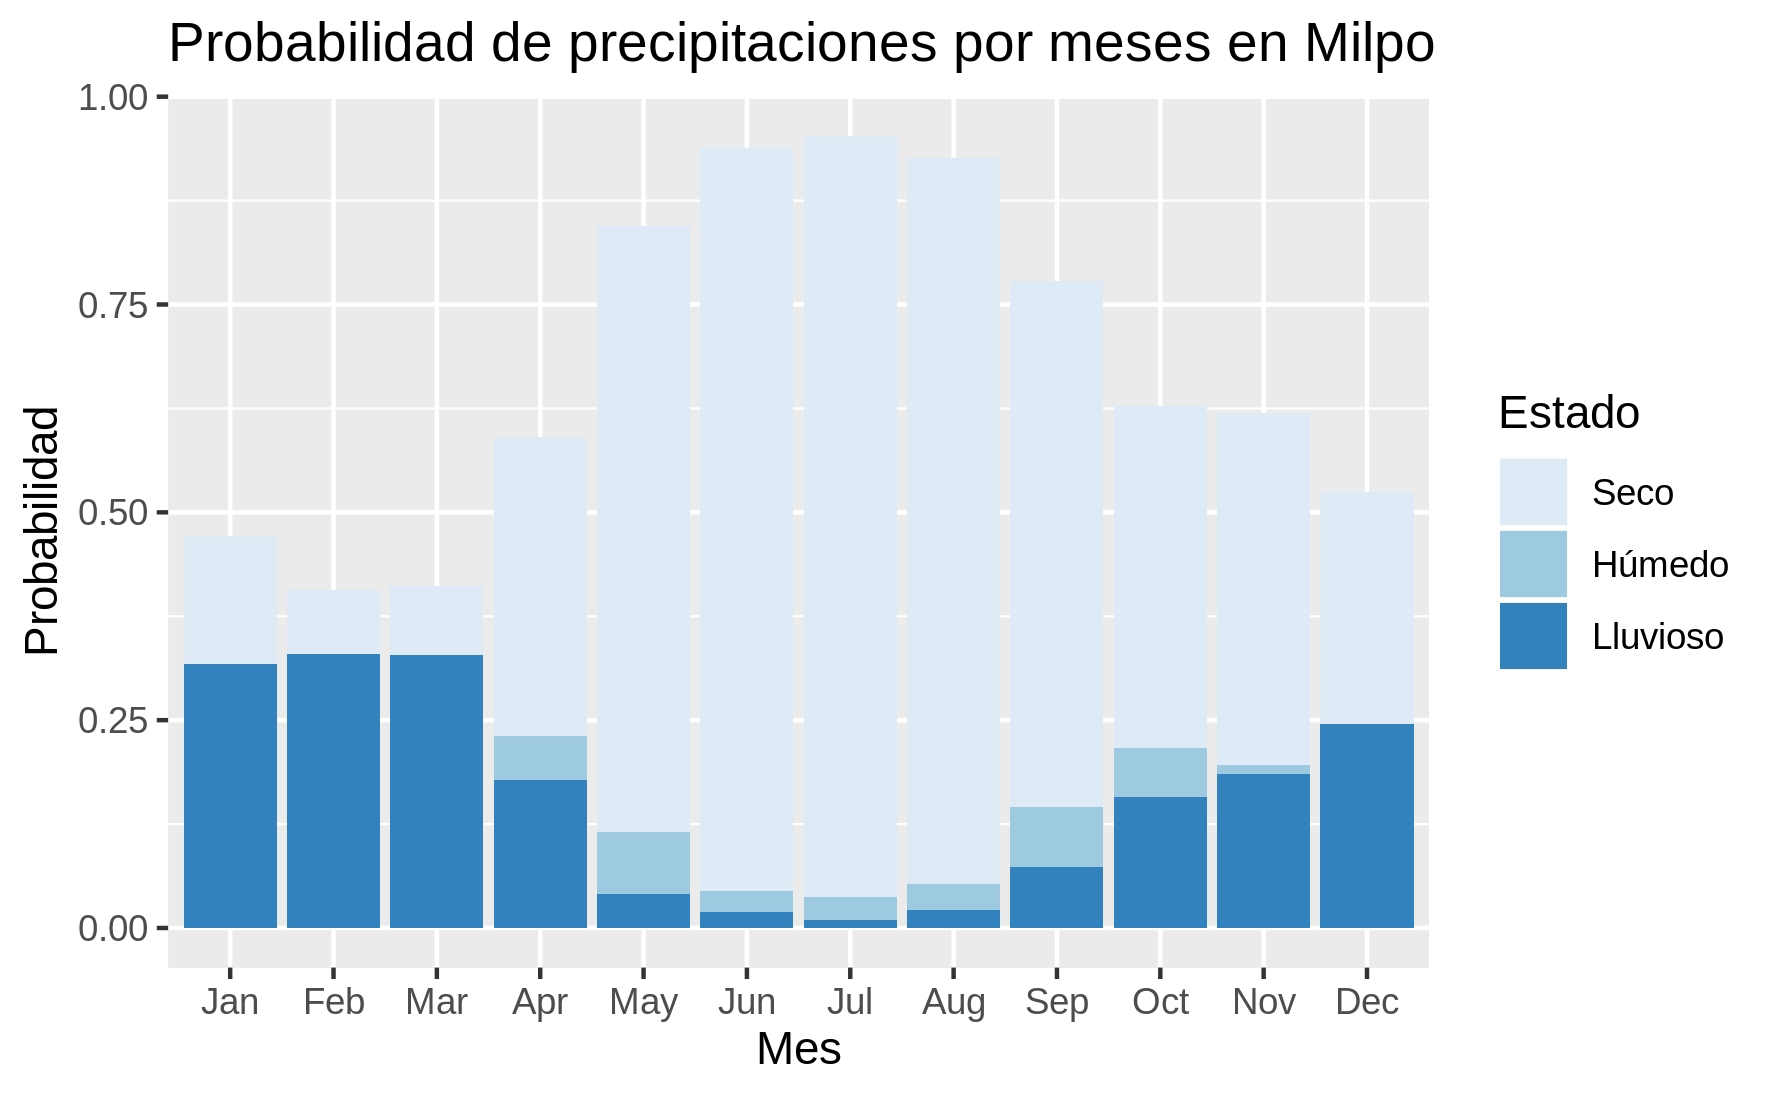
\includegraphics[width=\textwidth]{milpo.png}\\\\
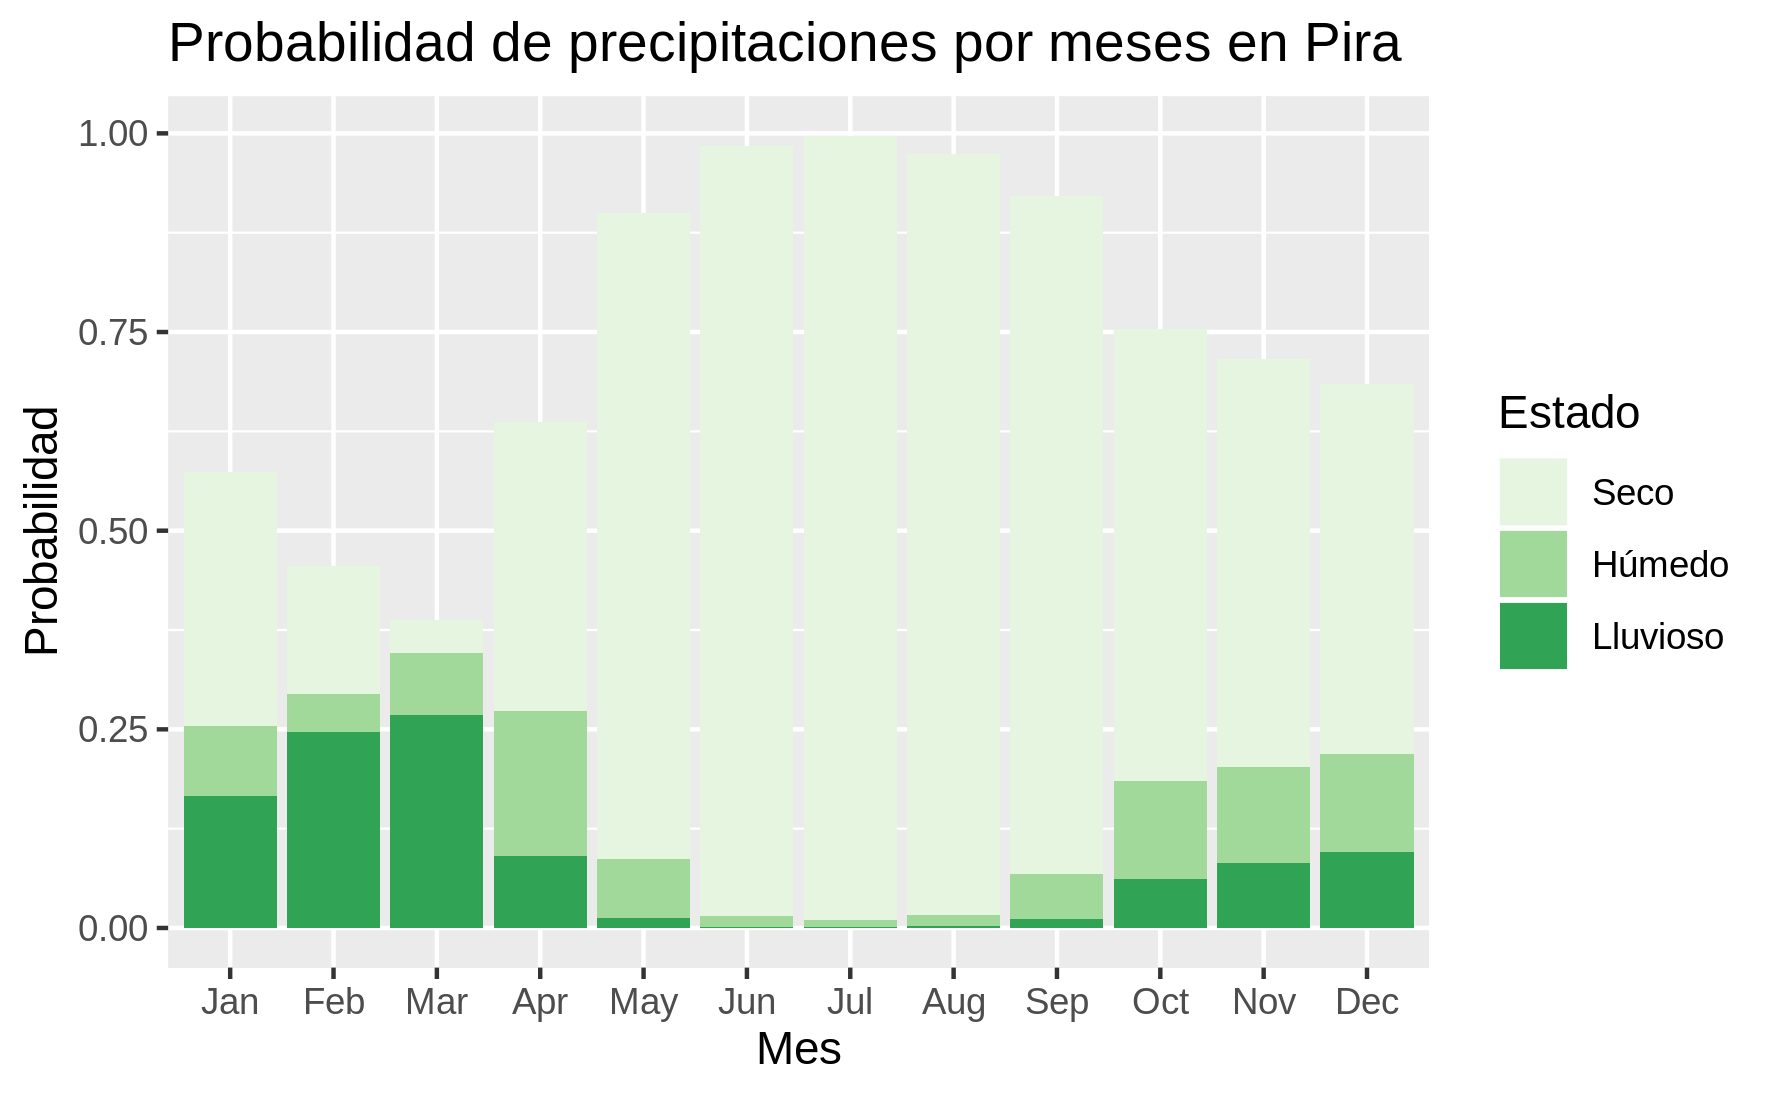
\includegraphics[width=\textwidth]{pira.png}\\\\
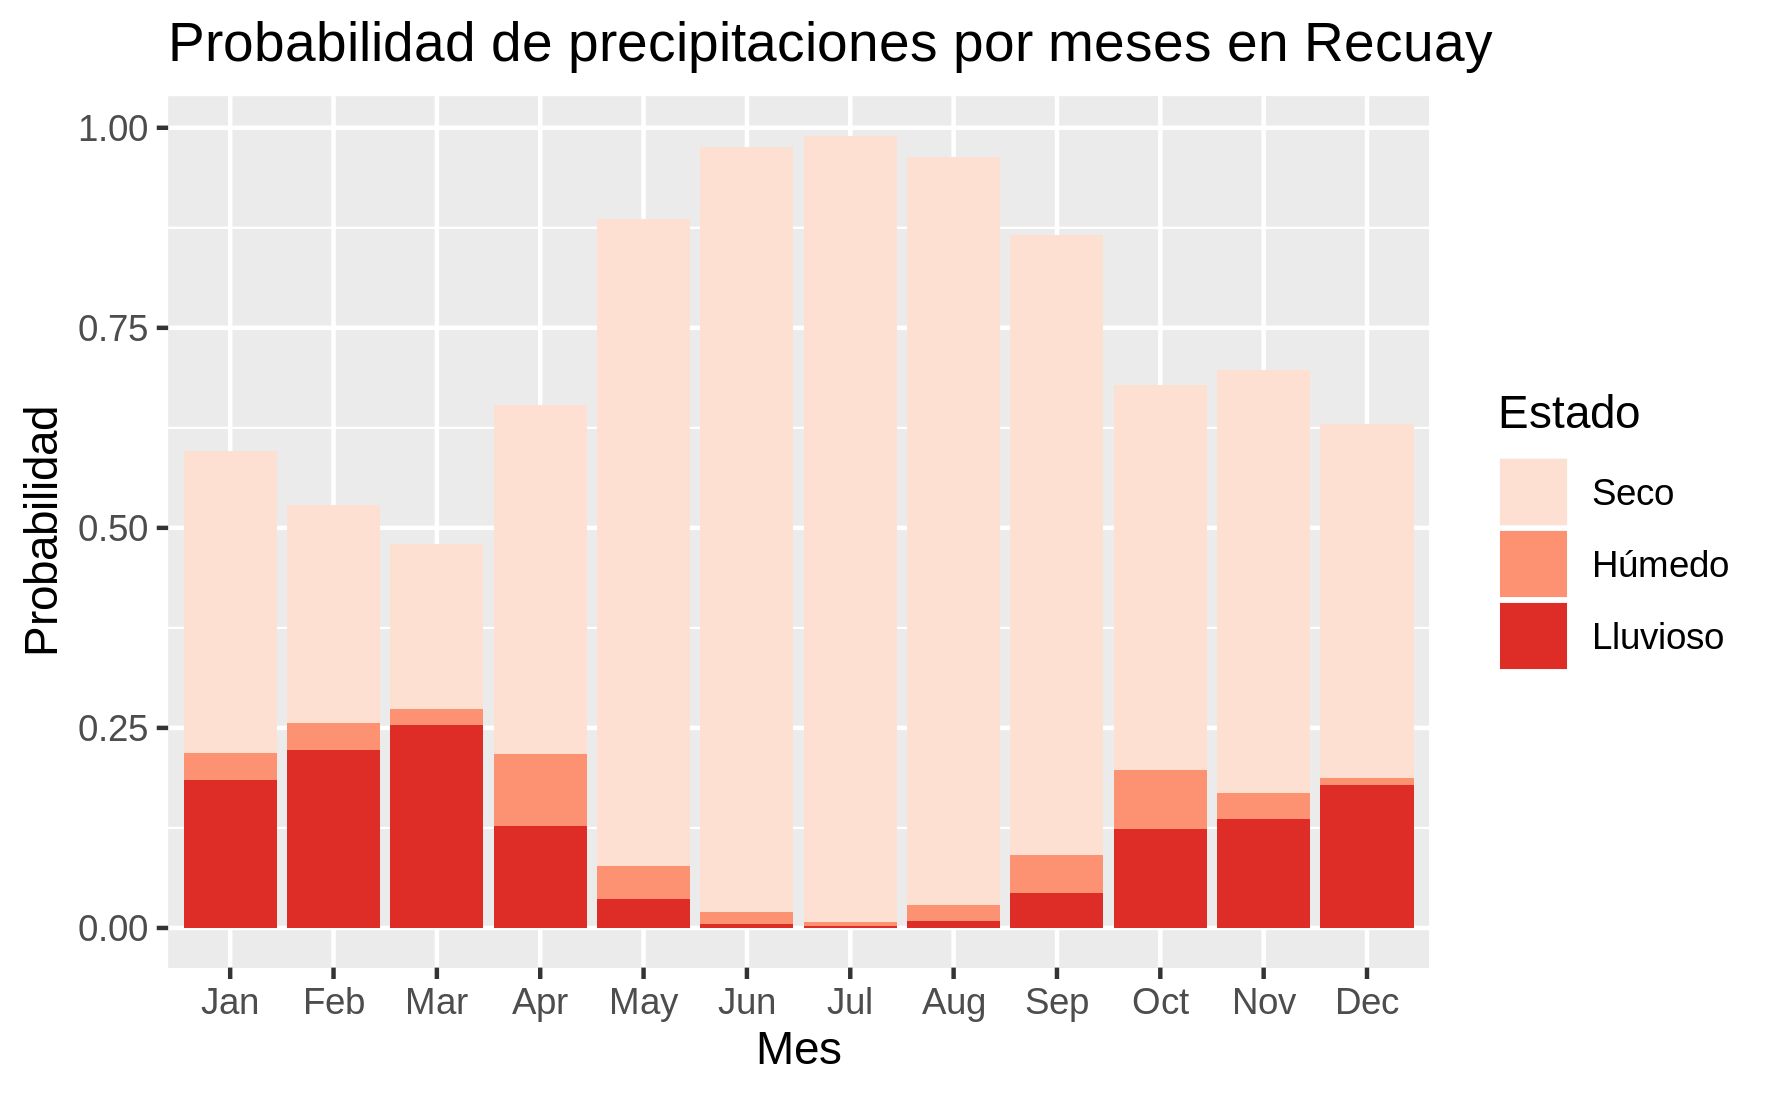
\includegraphics[width=\textwidth]{recuay.png}\\\\

\section{Conclusiones}

\begin{itemize}
    \item  Podemos notar que Milpo es la zona donde hay mayor probabilidad de lluvias durante los meses de siembra (enero-marzo), por lo que sería conveniente sembrar en esta zona productos que requieran grandes cantidades de recursos hídricos.
    \item Recuay y Pira también poseen lluvias de moderada a fuerte intensidad en los mismos meses, pero no en la misma proporción.
    \item Observando ambas gráficas se puede observar que los resulatados obtenidos por la simulación son muy similares a los datos originales, por lo que el modelo de Márkov simulo las precipitaciones y estados futuros con éxito.
\end{itemize}
\newpage
\section{Referencias}

\begingroup
\renewcommand{\section}[2]{}%
%\renewcommand{\chapter}[2]{}% for other classes

\begin{thebibliography}{..}

\bibitem{}
Khadr, M. (2016, 03). Forecasting of meteorological drought using Hidden Markov Model (case study: The upper Blue Nile river basin, Ethiopia). Ain Shams Engineering Journal, 7(1), 47-56.\\ doi:10.1016/j.asej.2015.11.005
\bibitem{}
Tettey, M., Oduro, F. T., Adedia, D., \& Abaye, D. A. (2017, 08). Markov chain analysis of the rainfall patterns of five geographical locations in the south eastern coast of Ghana. Earth Perspectives, 4(1). \\
Doi:10.1186/s40322-017-0042-6
\bibitem{}
Yoo, C., Lee, J., \& Ro, Y. (2016). Markov Chain Decomposition of Monthly Rainfall into Daily Rainfall: Evaluation of Climate Change Impact. Advances in Meteorology, 2016, 1-10.\\ Doi:10.1155/2016/7957490
\bibitem{}
Yusuf, A. U. (2014). Markov Chain Model and Its Application to Annual Rainfall Distribution for Crop Production. American Journal of Theoretical and Applied Statistics, 3(2), 39. doi:10.11648/j.ajtas.20140302.12

\end{thebibliography}

\endgroup


\end{document}
